\documentclass[11pt,a4paper]{article}

\usepackage[margin=1in]{geometry}
\usepackage{listings}
\usepackage{xcolor}
\usepackage{hyperref}
\usepackage{enumitem}
\usepackage{amsmath}
\usepackage{amssymb}
\usepackage{booktabs}
\usepackage{graphicx}
\usepackage{tikz}
\usetikzlibrary{arrows.meta, positioning, shapes.geometric, fit, calc}

\hypersetup{colorlinks=true, linkcolor=blue!70!black, urlcolor=blue!70!black}

\definecolor{codebg}{RGB}{245,245,245}
\definecolor{keyword}{RGB}{0,100,180}
\definecolor{comment}{RGB}{100,100,100}
\definecolor{string}{RGB}{180,0,0}

\lstdefinestyle{mlir}{
  backgroundcolor=\color{codebg},
  basicstyle=\ttfamily\small,
  keywordstyle=\color{keyword}\bfseries,
  commentstyle=\color{comment}\itshape,
  stringstyle=\color{string},
  breaklines=true,
  frame=single,
  rulecolor=\color{gray!30},
  morekeywords={air, channel, put, get, herd, segment, launch, token, memcpy,
    wait, wait_all, async, scf, for, parallel, yield, memref, alloc, linalg,
    matmul, arith, addi, constant},
  literate={->}{$\rightarrow$}1,
  xleftmargin=1em,
  framexleftmargin=0.5em,
}
\lstset{style=mlir}

\title{\textbf{MLIR-AIR: From Loop Nests to Silicon}\\[0.5em]
\large Detailed Notes on Mapping AI Workloads onto AMD NPUs}
\author{Adithya Jillellamudi}
\date{September 2026}

\begin{document}
\maketitle
\tableofcontents
\newpage

% =============================================================================
\section{What is MLIR-AIR?}
% =============================================================================

MLIR-AIR is a new MLIR dialect that bridges the gap between high-level AI workloads
(written in PyTorch, TensorFlow, Triton) and fine-grained spatial architectures like
AMD's NPUs. The key idea: traditional compiler IRs hide parallelism, data movement,
and synchronization behind abstractions like shared memory and thread schedulers.
Spatial hardware has none of that---no caches, no coherence, no central scheduler.
AIR makes all three \textbf{explicit in the IR itself}.

Three things AIR exposes that traditional IRs hide:

\begin{enumerate}[leftmargin=2em]
  \item \textbf{Spatial structure} --- \emph{where} computation runs (which tile,
    which core, which region of the chip). Expressed via \texttt{air.herd} and
    \texttt{air.segment}.
  \item \textbf{Temporal structure} --- \emph{when} things happen. Expressed via
    \texttt{air.token} dependency edges, not implicit memory ordering.
  \item \textbf{Data movement as first-class operations} ---
    \texttt{air.channel.put}/\texttt{air.channel.get} are separate IR ops. Compiler
    can see, schedule, and overlap them with compute.
\end{enumerate}

\subsection{Frontend Stays the Same}

AIR does \emph{not} change the programming model. The pipeline is:

\begin{center}
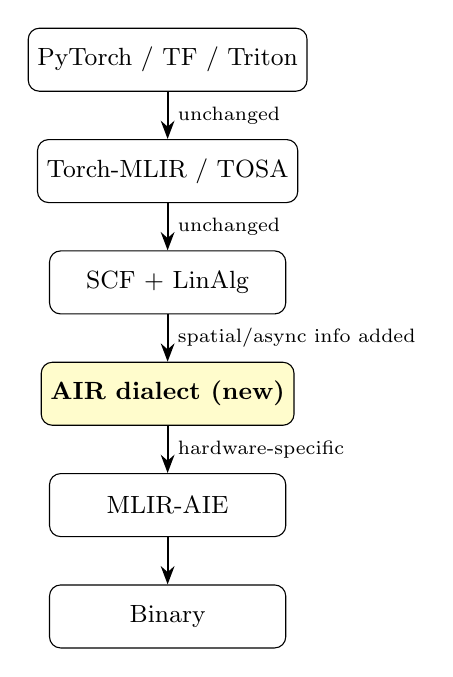
\begin{tikzpicture}[
  box/.style={draw, rounded corners, minimum width=3cm, minimum height=0.8cm,
    align=center, font=\small},
  arrow/.style={-{Stealth}, thick},
  node distance=0.6cm
]
\node[box] (pt) {PyTorch / TF / Triton};
\node[box, below=of pt] (torch) {Torch-MLIR / TOSA};
\node[box, below=of torch] (scf) {SCF + LinAlg};
\node[box, below=of scf, fill=yellow!20] (air) {\textbf{AIR dialect (new)}};
\node[box, below=of air] (aie) {MLIR-AIE};
\node[box, below=of aie] (bin) {Binary};

\draw[arrow] (pt) -- (torch) node[midway, right, font=\scriptsize] {unchanged};
\draw[arrow] (torch) -- (scf) node[midway, right, font=\scriptsize] {unchanged};
\draw[arrow] (scf) -- (air) node[midway, right, font=\scriptsize]
  {spatial/async info added};
\draw[arrow] (air) -- (aie) node[midway, right, font=\scriptsize]
  {hardware-specific};
\draw[arrow] (aie) -- (bin);
\end{tikzpicture}
\end{center}

AIR is a \textbf{new middle layer} inserted between generic MLIR and hardware-specific
MLIR-AIE. It doesn't change anything above it. The compiler \emph{infers} spatial
structure from loop nests and tiling decisions, then \emph{encodes} it as AIR operations.


% =============================================================================
\section{Why Spatial Hardware Needs a New IR}
% =============================================================================

\subsection{Standard IR vs.\ AIR: The Core Difference}

Standard IRs (LLVM IR, MLIR SCF+memref) model programs as:
\begin{itemize}[leftmargin=2em]
  \item \textbf{Shared memory} --- all threads see one big address space. Write to
    address X, any thread reads X. Hardware caches and coherence protocols make this
    work.
  \item \textbf{Centralized scheduling} --- you say ``run 1000 threads.'' One
    scheduler (OS on CPU, warp scheduler on GPU) maps threads to cores. You don't
    control placement.
\end{itemize}

In this model, the IR looks like:
\begin{lstlisting}
%val = memref.load %buf[%i]     // which memory? don't care
%res = arith.muli %val, %val    // on which core? don't care
memref.store %res, %out[%i]     // when visible? hardware sorts it out
\end{lstlisting}

No information about where things physically are, who moves data, or what depends on
what (beyond program order).

AIR flips this. Same operation in AIR:
\begin{lstlisting}
%tok0 = air.channel.get %L1_buf from @chan_A  // explicit DMA: L2 -> L1
air.herd [%x, %y] in [4, 4] {                // explicit: 4x4 cores
    %tok1 = air.wait %tok0                    // explicit: wait for DMA
    linalg.matmul %L1_A, %L1_B, %L1_C        // compute on local data
    air.channel.put %L1_C to @chan_out        // explicit DMA: L1 -> L2
}
\end{lstlisting}

Every question the standard IR leaves to hardware---\emph{where} is the data,
\emph{who} moves it, \emph{which cores} compute, \emph{what} waits for
\emph{what}---AIR answers explicitly.

\subsection{Why Standard IR Can't Target Spatial Hardware}

If you give a spatial NPU code that says ``load from memory,'' the hardware doesn't
know which memory, through which path, into which scratchpad. There's no cache.
No coherence. No central scheduler. The IR \emph{must} carry this information or the
backend has nothing to work with.


% =============================================================================
\section{Hardware Trends Motivating AIR}
% =============================================================================

\subsection{Multi-root Memory Hierarchy (NUMA at Chip Scale)}

Traditional compilers treat main memory as one coherent root. Modern devices use
multiple independent memory channels for aggregate bandwidth. These channels are
\emph{physically separate paths to different parts of memory}. No hardware coherence
between them.

\textbf{Example:} Matrix multiply on a multi-chiplet NPU. Matrix B shared across
cores. B lives behind chiplet 0's memory channel.
\begin{itemize}[leftmargin=2em]
  \item Chiplet 0 reads B fast---local channel, short path
  \item Chiplet 1 reads same B \textbf{slow}---across interconnect, contends for
    chiplet 0's memory port
\end{itemize}

Even with co-design, NUMA effects creep in at scale because:
\begin{itemize}[leftmargin=2em]
  \item \textbf{Wire delay scales with distance.} Core at top-left of a 10$\times$10
    grid is far from memory at bottom-right ($\sim$1cm/ns on silicon).
  \item \textbf{Bandwidth is finite.} One memory port can't feed 100 cores. Partition
    into banks $\Rightarrow$ non-uniform access.
  \item \textbf{Multi-chiplet is often necessary.} Yield drops with die size, so
    chiplets connected by inter-chiplet links (slower than on-die wires).
\end{itemize}

\subsection{DMA: Mechanism vs.\ Policy}

DMA \emph{moves} data but doesn't \emph{decide} what to move, when, or where.

\begin{enumerate}[leftmargin=2em]
  \item \textbf{DMA doesn't know about duplicates.} 8 cores needing tile B: naive
    compiler issues 8 DMAs from remote memory. Smart compiler: one DMA to local
    memory, 8 local reads.
  \item \textbf{DMA doesn't schedule itself.} Fire too late $\Rightarrow$ cores stall.
    Too early $\Rightarrow$ local buffer overflow. Compiler must pipeline prefetches.
  \item \textbf{DMA doesn't know topology.} Two DMAs sharing a path contend.
    DMA engine doesn't throttle across channels.
\end{enumerate}

The compiler is the logistics planner; DMA is the truck. AIR models the topology so
the compiler can make good placement/scheduling decisions.

\subsection{Asynchronous Execution}

Each NPU tile has multiple \textbf{independent actors}:
\begin{itemize}[leftmargin=2em]
  \item \textbf{Compute engine} --- vector/scalar ALU
  \item \textbf{DMA engine} --- moves data between memory levels
  \item \textbf{NoC switch} --- routes data between tiles
\end{itemize}

These operate concurrently. Naive sequential execution wastes half the time (one actor
idle while another works). Async execution pipelines them:

\begin{center}
\begin{tabular}{lccc}
\toprule
& DMA get & Compute & DMA put \\
\midrule
Iter 0 & \texttt{[====]} & \texttt{[====]} & \texttt{[====]} \\
Iter 1 & \quad\texttt{[====]} & \quad\texttt{[====]} & \quad\texttt{[====]} \\
Iter 2 & \qquad\texttt{[====]} & \qquad\texttt{[====]} & \qquad\texttt{[====]} \\
\bottomrule
\end{tabular}
\end{center}

Each actor has a local hardware scheduler with a task queue. When a dependency is
satisfied (token fires), it picks next task. No central coordinator.
\texttt{air.token} encodes these dependencies in the IR.


% =============================================================================
\section{Four Compiler Requirements for Spatial Hardware}
% =============================================================================

The paper identifies four capabilities a compiler framework must have (Section~2.2):

\begin{enumerate}[leftmargin=2em]
  \item \textbf{Memory allocation control.} Allocate memory at specific levels
    (L1/L2/DRAM) \emph{and} specific NUMA domains within each level.
    Not just \texttt{malloc(size)} but ``put this in L1 of tile (2,3)'' or
    ``L2 of cluster 0.''
    In AIR: \texttt{memref} types with memory space annotations.

  \item \textbf{Compute placement control.} Describe which cores form a group,
    run concurrently, share resources for cheap sync.
    In AIR: \texttt{air.herd} places compute on a core grid,
    \texttt{air.segment} groups herds sharing resources.

  \item \textbf{Separate data movement from computation.} Make DMA ops visible
    in the IR so compiler can schedule them independently, overlap with compute,
    apply architecture-specific optimizations.
    In AIR: \texttt{air.channel.put}/\texttt{get} are separate IR nodes.

  \item \textbf{Dependency resolution close to hardware.} Express dependencies
    explicitly so hardware resolvers (not software polling) can react in nanoseconds.
    In AIR: \texttt{air.token} values $\rightarrow$ lowered to hardware lock signals
    on tile task queues.
\end{enumerate}


% =============================================================================
\section{Comparison with Related Frameworks}
% =============================================================================

\subsection{IRON: Close-to-Metal Toolkit}

IRON is a Python toolkit for AMD NPUs. You manually control everything: tile
placement, DMA configuration, synchronization locks. Key abstraction:
\texttt{ObjectFifo}---a circular buffer between producer and consumer with built-in
lock synchronization.

\begin{center}
\begin{tabular}{lll}
\toprule
& \textbf{IRON} & \textbf{AIR} \\
\midrule
Abstraction level & Assembly-like & C-like \\
Placement & Manual & Compiler-managed \\
DMA config & Hand-written descriptors & Compiler-inferred \\
Target & Single kernels & Complex fused workloads \\
IR level & \texttt{mlir-aie} (bottom) & AIR dialect (middle) \\
\bottomrule
\end{tabular}
\end{center}

Both target the same \texttt{mlir-aie} backend. AIR automates what IRON makes
you do by hand. IRON is for peak performance on small kernels; AIR makes complex
workloads (like full attention blocks, $\sim$150 lines) feasible.

\subsection{ARIES: Agile Compilation Flow}

ARIES is an MLIR-based compilation flow for AIE architectures with a Triton-like
programming model (tile-based task abstraction with scheduling primitives like
\texttt{.to()}, \texttt{.pipeline()}, \texttt{.vectorize()}).

ARIES is modular: unified MLIR IR covering AIE core, AIE array, and PL (FPGA),
with portable backends for both Versal ACAP and Ryzen NPU. It reuses existing MLIR
dialects (SCF, memref, affine, AIEVec, ADF).

\textbf{The paper's specific distinction:} ARIES's spatial intelligence lives in the
\emph{frontend API} (Python scheduling primitives) and \emph{lowering pipeline}.
AIR encodes spatial/async semantics as \emph{new IR operations}
(\texttt{air.herd}, \texttt{air.channel}, \texttt{air.token}) visible to any MLIR
pass. Whether this distinction matters practically is debatable---both achieve good
GEMM results.


% =============================================================================
\section{ACDG: Asynchronous Control and Dataflow Graph}
% =============================================================================

\subsection{What It Is}

A DAG embedded directly in the MLIR-AIR IR:
\begin{itemize}[leftmargin=2em]
  \item \textbf{Nodes} = MLIR operations (compute, DMA, sync)
  \item \textbf{Edges} = dependencies encoded via \texttt{air.token} SSA values
\end{itemize}

Not a separate data structure. Uses MLIR's native SSA (Static Single Assignment)
form: every \texttt{air.token} value is defined exactly once, and any operation
consuming it must be dominated by its definition. MLIR's existing verifier checks
dependency correctness \emph{for free}.

\subsection{Token Mechanism}

An operation marked \texttt{async} \textbf{produces} a token. An operation that
\textbf{consumes} that token can't execute until the producer finishes:

\begin{lstlisting}
%tok0 = air.channel.get async @chan, %buf   // produces tok0
%tok1 = linalg.matmul async [%tok0] ...     // waits for tok0
%tok2 = air.channel.put async [%tok1] ...   // waits for tok1
\end{lstlisting}

Independent ops have no edge $\Rightarrow$ run in parallel:
\begin{lstlisting}
%tok0 = air.channel.get async @chanA, %bufA  // fetch A
%tok1 = air.channel.get async @chanB, %bufB  // fetch B (no dep on tok0!)
%tok2 = linalg.matmul async [%tok0, %tok1]   // waits for BOTH
\end{lstlisting}

\subsection{Dependency Types (RAW, WAR, WAW)}

Three classic data hazards, all encoded as token edges:

\begin{description}[leftmargin=2em]
  \item[RAW (Read After Write):] Compute reads buffer after DMA writes it.
    Most common. Must wait for write to complete.
  \item[WAR (Write After Read):] DMA overwrites buffer with next tile while
    compute still reading current tile. Must wait for read to finish.
  \item[WAW (Write After Write):] Two DMAs writing same buffer. Second waits
    for first to avoid corruption.
\end{description}

\subsection{Why CPU Hazard Resolution Fails on NPUs}

On CPUs, RAW/WAR/WAW are resolved \emph{at runtime by hardware}:

\begin{description}[leftmargin=2em]
  \item[Data forwarding / bypassing:] Result from ALU output is wired directly to
    a dependent instruction's input, skipping register writeback. Requires a
    centralized pipeline with bypass muxes between stages.
  \item[Tomasulo / register renaming:] WAR and WAW disappear by mapping
    architectural registers to a larger pool of physical registers. Each write
    targets a fresh physical register; concurrent reads of the old value are safe.
    Requires a centralized rename table and scoreboard.
  \item[Reorder buffer (ROB):] Allows out-of-order execution with in-order
    commit. Requires centralized tracking of all in-flight operations.
\end{description}

\textbf{None of these transfer to spatial architectures:}
\begin{itemize}[leftmargin=2em]
  \item \textbf{No central pipeline.} Data lives in distributed scratchpads across
    physically separate tiles. Cannot ``forward'' a 4KB buffer across a NoC the
    way a CPU forwards a 64-bit value through a bypass mux.
  \item \textbf{No centralized register file.} The ``registers'' are tile-local
    SRAM buffers managed by the compiler, not a hardware rename unit. No
    scoreboard watches all tiles simultaneously.
  \item \textbf{Wire delay at spatial scale.} A centralized ROB would need global
    visibility across dozens of independent tiles, each running its own DMA engine
    and compute engine. Physically impractical.
\end{itemize}

\textbf{NPU resolution: compile-time token edges.} The ACDG resolves all three
hazards \emph{statically}. The compiler determines ordering and inserts
\texttt{air.token} SSA values that create happens-before constraints (paper p.25--26:
dependencies ``encoded directly in the IR using SSA token values''). Hardware simply
obeys the token ordering---when a token is not yet produced, the dependent op waits.
No speculation, no dynamic reordering.

\begin{center}
\small
\begin{tabular}{lll}
\toprule
& \textbf{CPU} & \textbf{NPU (AIR)} \\
\midrule
When resolved & Runtime (hardware) & Compile time (compiler) \\
RAW & Data forwarding & Token edge: DMA$\rightarrow$compute \\
WAR & Register renaming & Token edge: compute$\rightarrow$next DMA \\
WAW & Register renaming & Token edge: DMA$\rightarrow$DMA \\
Mechanism & Bypass mux, rename table, ROB & \texttt{air.token} SSA values \\
Why it works & Dynamic ILP extraction & Workload is regular, predictable \\
\bottomrule
\end{tabular}
\end{center}

This is why the paper argues the compiler needs ``dependency resolution close to
hardware'' (requirement~4, p.12)---the hardware will not solve it for you.

\subsection{Three Kinds of Synchronization Edges}

From Section 5.3.1 (p.12), the compute model defines three relationship types
between operations controlled by synchronization lists:

\begin{enumerate}[leftmargin=2em]
  \item \textbf{Dependency lists} --- \emph{directed} edges. ``A must finish before B
    starts'' (happens-before). Encodes RAW/WAR/WAW hazards. Paper: ``requires
    that all inputs to a operation that are modified by a source operation in the
    dependency list are visible before the sink operation is scheduled.''
  \item \textbf{Concurrency lists} --- \emph{undirected} edges. ``A and B must run at
    the same time'' on exclusive resources. Paper: ``each \texttt{air.token}
    in a concurrency list defines an undirected edge between two operations that
    indicates they must be scheduled at the same time. This implies that each
    operation must use exclusive resources.''
  \item \textbf{Affinity lists} --- \emph{undirected} edges. ``A and B must use the same
    physical resources'' but at \emph{different} times. Paper: ``these operations'
    time-slots must be disjoint, but the edge does not describe which operation
    must be scheduled first.''
\end{enumerate}

\subsubsection{Concrete Example: Double-Buffered Matmul Tile}

Consider one tile computing $C \mathrel{+}= A \times B$ across two iterations with
double buffering. Each iteration has four operations:

\begin{center}
\small
\begin{tabular}{lll}
\toprule
\textbf{Op} & \textbf{Iteration 0} & \textbf{Iteration 1} \\
\midrule
Fetch A tile (L2$\rightarrow$L1) & \texttt{DMA\_A0} & \texttt{DMA\_A1} \\
Fetch B tile (L2$\rightarrow$L1) & \texttt{DMA\_B0} & \texttt{DMA\_B1} \\
Compute matmul & \texttt{Comp0} & \texttt{Comp1} \\
Write C tile (L1$\rightarrow$L2) & \texttt{DMA\_C0} & \texttt{DMA\_C1} \\
\bottomrule
\end{tabular}
\end{center}

The ACDG for this scenario contains all three edge types:

\begin{center}
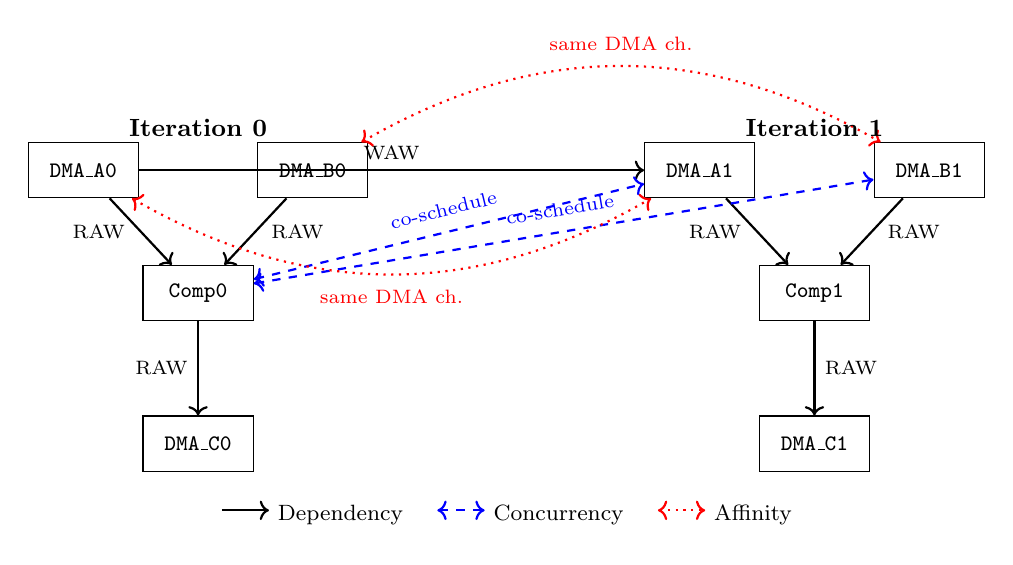
\begin{tikzpicture}[
    op/.style={rectangle, draw, minimum width=1.4cm, minimum height=0.7cm,
               font=\footnotesize\ttfamily},
    dep/.style={->, thick},
    conc/.style={<->, dashed, thick, blue},
    aff/.style={<->, dotted, thick, red},
    every node/.style={font=\footnotesize},
    node distance=1.2cm and 2.0cm
]
% Iteration 0
\node[op] (da0) {DMA\_A0};
\node[op, right=1.5cm of da0] (db0) {DMA\_B0};
\node[op, below=1.2cm of $(da0)!0.5!(db0)$] (c0) {Comp0};
\node[op, below=1.2cm of c0] (dc0) {DMA\_C0};

% Iteration 1
\node[op, right=3.5cm of db0] (da1) {DMA\_A1};
\node[op, right=1.5cm of da1] (db1) {DMA\_B1};
\node[op, below=1.2cm of $(da1)!0.5!(db1)$] (c1) {Comp1};
\node[op, below=1.2cm of c1] (dc1) {DMA\_C1};

% Dependency edges (solid arrows) -- within iteration
\draw[dep] (da0) -- (c0) node[midway, left, xshift=-2pt] {\scriptsize RAW};
\draw[dep] (db0) -- (c0) node[midway, right, xshift=2pt] {\scriptsize RAW};
\draw[dep] (c0) -- (dc0) node[midway, left] {\scriptsize RAW};
\draw[dep] (da1) -- (c1) node[midway, left, xshift=-2pt] {\scriptsize RAW};
\draw[dep] (db1) -- (c1) node[midway, right, xshift=2pt] {\scriptsize RAW};
\draw[dep] (c1) -- (dc1) node[midway, right] {\scriptsize RAW};

% Dependency edge -- cross-iteration (WAW: same buffer reuse)
\draw[dep] (da0) -- (da1) node[midway, above] {\scriptsize WAW};

% Concurrency edges (dashed blue) -- double buffering overlap
\draw[conc] (c0) -- (da1) node[midway, above, sloped, yshift=2pt]
    {\scriptsize co-schedule};
\draw[conc] (c0) -- (db1) node[midway, above, sloped, yshift=2pt]
    {\scriptsize co-schedule};

% Affinity edges (dotted red) -- same physical DMA channel
\draw[aff, bend right=30] (da0) to
    node[midway, below, sloped, yshift=-2pt] {\scriptsize same DMA ch.} (da1);
\draw[aff, bend left=30] (db0) to
    node[midway, above, sloped, yshift=2pt] {\scriptsize same DMA ch.} (db1);

% Labels
\node[above=0.3cm of $(da0)!0.5!(db0)$, font=\small\bfseries] {Iteration 0};
\node[above=0.3cm of $(da1)!0.5!(db1)$, font=\small\bfseries] {Iteration 1};

% Legend
\node[below=0.6cm of $(dc0)!0.5!(dc1)$, anchor=north] (leg) {
  \begin{tabular}{lll}
    {\tikz\draw[dep] (0,0)--(0.6,0);} Dependency &
    {\tikz\draw[conc] (0,0)--(0.6,0);} Concurrency &
    {\tikz\draw[aff] (0,0)--(0.6,0);} Affinity
  \end{tabular}
};
\end{tikzpicture}
\end{center}

\textbf{Reading the diagram:}
\begin{itemize}[leftmargin=2em]
  \item \textbf{Solid arrows (dependency):}
    \texttt{DMA\_A0}$\rightarrow$\texttt{Comp0} is a RAW edge: compute can't
    start until the DMA finishes writing the A tile into L1.
    \texttt{DMA\_A0}$\rightarrow$\texttt{DMA\_A1} is a WAW edge: both write to
    the same L1 buffer (buf\_A), so iteration~1's fetch must wait until
    iteration~0's fetch is consumed.

  \item \textbf{Dashed blue (concurrency):}
    \texttt{Comp0}$\leftrightarrow$\texttt{DMA\_A1} means these \emph{must}
    run simultaneously---this is double buffering. While the compute engine
    processes tile~0's data, the DMA engine fetches tile~1's data into the
    \emph{other} buffer. They use \textbf{exclusive} resources (compute engine
    vs.\ DMA engine), so no conflict. Without this edge, the scheduler could
    serialize them, killing the overlap.

  \item \textbf{Dotted red (affinity):}
    \texttt{DMA\_A0}$\leftrightarrow$\texttt{DMA\_A1} means both must use the
    \emph{same physical DMA channel}, but at different times. The compiler uses
    this to allocate DMA channels: these two ops share a channel, not compete for
    separate ones. Time-slots are disjoint (guaranteed by the WAW dependency
    edge), but the resource binding is the same.
\end{itemize}

\subsubsection{Why Three Edges, Not Just Dependency?}

Dependency alone can express \emph{ordering} but not \emph{resource binding} or
\emph{co-scheduling}. A compiler that only has dependency edges would:
\begin{itemize}[leftmargin=2em]
  \item Miss the double-buffering overlap (concurrency): it would see
    \texttt{DMA\_A1} has no dependency on \texttt{Comp0} and might schedule it
    \emph{before} or \emph{after}---but not constrain it to run \emph{during}.
  \item Allocate DMA channels independently per operation (affinity): without
    knowing that \texttt{DMA\_A0} and \texttt{DMA\_A1} should reuse the same
    channel, it might allocate two channels or fail to reuse hardware.
\end{itemize}

\subsection{Composing with Loops: Software Pipelining}

Tokens as \texttt{scf.for} iteration arguments enable software pipelining:

\begin{lstlisting}
scf.for %i = 0 to N iter_args(%prev_dma = %init_tok) {
    %tok0 = air.channel.get async [%prev_dma] -> %buf
    %tok1 = matmul async [%tok0]
    %tok2 = air.channel.put async [%tok1]
    scf.yield %tok0    // next iter's DMA waits only for this DMA
}
\end{lstlisting}

Key: iteration $i{+}1$'s DMA waits only for iteration $i$'s DMA (via
\texttt{\%prev\_dma}), \emph{not} for $i$'s compute or store:

\begin{center}
\begin{tabular}{llll}
\toprule
& DMA\_get & compute & DMA\_put \\
\midrule
Iter 0: & \texttt{[====]} & \texttt{\quad[====]} & \texttt{\qquad[====]} \\
Iter 1: & \texttt{\quad[====]} & \texttt{\qquad[====]} & \texttt{\quad\qquad[====]} \\
Iter 2: & \texttt{\qquad[====]} & \texttt{\quad\qquad[====]} & \\
\bottomrule
\end{tabular}
\end{center}

The pipeline overlap is expressed purely through which token gets passed as
the loop-carried argument. Compiler sees the graph structure and can optimize
pipeline depth and buffer allocation.


% =============================================================================
\section{AIR Dialect Constructs in Use: Vector-Add Walkthrough}
% =============================================================================

The paper (Section~6, p.13; Listing~7, p.33; Listing~3, p.14) demonstrates AIR on
an element-wise vector add. This section starts from the plain algorithm, shows what
the generic IR looks like, explains what's missing, then walks through the AIR output
stage by stage.

% ---- Stage 0: The Algorithm ----
\subsection{Stage 0: The Algorithm (What We Actually Want to Compute)}

\begin{lstlisting}
// Element-wise vector add: out[i] = in1[i] + in2[i]
// 65536 float32 elements
for i in range(65536):
    out[i] = in1[i] + in2[i]
\end{lstlisting}

That's it. Three arrays, one loop, one add per element. 65536 $\times$ 4 bytes =
256\,KB per array, 768\,KB total. No parallelism expressed, no tiling, no memory
hierarchy---just the math.

\textbf{The question}: how does this get from a flat loop to running on a spatial
NPU with distributed memories, DMA engines, and parallel tiles? Two stages:
\begin{enumerate}[leftmargin=2em]
  \item \textbf{Generic MLIR} (Listing~7): upstream frameworks (Torch-MLIR, Triton)
    lower it to standard MLIR dialects with tiling and parallelism, but no spatial
    awareness.
  \item \textbf{AIR IR} (Listing~3): MLIR-AIR transforms that into a fully spatial,
    async, explicitly-scheduled program.
\end{enumerate}


% ---- Stage 1: Generic MLIR ----
\subsection{Stage 1: Generic MLIR Input (Listing~7, p.33)}

The upstream compiler has already done two things to the flat loop:
\textbf{parallelized} it (split into 2 independent halves) and \textbf{tiled} it
(process 1024 elements at a time into local buffers). But it uses only standard MLIR
dialects (SCF, MemRef, Arith)---no spatial constructs. Paper p.13: ``agnostic to the
target hardware and does not yet reflect spatial execution, memory locality, or
asynchronous scheduling.''

\subsubsection{Step 1: Function Signature --- Three Flat Buffers}
\begin{lstlisting}
func.func @eltwise_add(%arg0: memref<65536xf32>,   // in1
                        %arg1: memref<65536xf32>,   // in2
                        %arg2: memref<65536xf32>) { // out
\end{lstlisting}

Three flat 65536-element buffers. \texttt{memref<65536xf32>} = a pointer to
contiguous memory. No hierarchy info---all three live in ``some memory'' with no
distinction between host DRAM, L2, or L1 scratchpad.

\textbf{What's missing}: on the NPU, \texttt{in1} starts in host DRAM (L3), tiles of
it need to be in L2 (shared memory) and then L1 (tile-local scratchpad) before
compute can touch it. This IR doesn't express any of that.

\subsubsection{Step 2: Parallelization --- Split Work, But No Placement}
\begin{lstlisting}
%c2 = arith.constant 2 : index
scf.parallel (%arg3) = (%c0) to (%c2) step (%c1) {
\end{lstlisting}

\texttt{scf.parallel} with 2 iterations: each processes half the vector (32768
elements). This says ``these iterations are independent and \emph{may} run in
parallel.''

\textbf{What's missing}: \texttt{scf.parallel} is an \emph{abstract} parallelism
marker. It doesn't say:
\begin{itemize}[leftmargin=2em]
  \item \emph{Which cores?} No tile coordinates, no grid shape.
  \item \emph{How many?} A scheduler could run both iterations on one core
    sequentially---nothing prevents it.
  \item \emph{Where physically?} No contiguity or affinity constraints.
\end{itemize}

\subsubsection{Step 3: Tiling --- Local Buffers, But Opaque Memory}
\begin{lstlisting}
%alloc   = memref.alloc() : memref<1024xf32, 2>  // local buf for in1 tile
%alloc_0 = memref.alloc() : memref<1024xf32, 2>  // local buf for in2 tile
%alloc_1 = memref.alloc() : memref<1024xf32, 2>  // local buf for out tile
\end{lstlisting}

Three 1024-element local buffers. The \texttt{2} is a memory space annotation---in
generic MLIR this is just an integer tag. It hints ``not default address space'' but
carries \textbf{no semantic meaning}: the compiler doesn't know if \texttt{2} means
L1 scratchpad, L2 shared, or GPU shared memory.

\textbf{What's missing}: on the NPU, L1 scratchpad on tile (0,0) is physically
different from L1 on tile (0,1). A 1024$\times$4 = 4\,KB buffer must fit in the
tile's local SRAM. This IR can't express that constraint.

\subsubsection{Step 4: Data Movement --- Coupled, Single-Sided}
\begin{lstlisting}
scf.for %arg4 = %c0 to %c65536 step %c2048 {
    %subview = memref.subview %arg0[%offset][1024][1]
                  : memref<65536xf32> to memref<1024xf32>
    memref.copy %subview, %alloc
        : memref<1024xf32> to memref<1024xf32, 2>
\end{lstlisting}

\texttt{memref.subview} creates a window (pointer + offset) into the big array.
\texttt{memref.copy} copies 1024 elements from that window into the local buffer.

\textbf{What's missing}: \texttt{memref.copy} is \textbf{coupled}---one operation
names \emph{both} source and destination. The compiler can't separately reason about:
\begin{itemize}[leftmargin=2em]
  \item The ``send'' side (who pushes data onto the interconnect)
  \item The ``receive'' side (who pulls data into local memory)
  \item Which memory level each side lives at
  \item Whether the transfer is blocking or can overlap with compute
\end{itemize}

On the NPU, data movement from L3$\rightarrow$L2 is a different DMA engine from
L2$\rightarrow$L1. \texttt{memref.copy} collapses both into one opaque operation.

\subsubsection{Step 5: Compute --- Correct, But Sequential}
\begin{lstlisting}
scf.for %arg5 = %c0 to %c1024 step %c1 {
    %0 = memref.load %alloc[%arg5]    : memref<1024xf32, 2>
    %1 = memref.load %alloc_0[%arg5]  : memref<1024xf32, 2>
    %2 = arith.addf %0, %1 : f32
    memref.store %2, %alloc_1[%arg5]  : memref<1024xf32, 2>
}
\end{lstlisting}

Load from both input buffers, add, store to output buffer. 1024 iterations.
Mathematically identical to the original \texttt{out[i] = in1[i] + in2[i]}, just
operating on a tile.

\textbf{What's missing}: everything here is \textbf{synchronous}. Each load blocks
until complete. No overlap between this compute and any DMA. No tokens, no
dependency tracking.

\subsubsection{Step 6: Write-Back and Cleanup}
\begin{lstlisting}
    %subview_3 = memref.subview %arg2[%offset][1024][1] ...
    memref.copy %alloc_1, %subview_3    // result -> global
    memref.dealloc %alloc
    memref.dealloc %alloc_0
    memref.dealloc %alloc_1
  }   // end scf.for (tiling loop)
  scf.reduce
}     // end scf.parallel
\end{lstlisting}

Copy result tile back to global output, deallocate local buffers. Again,
\texttt{memref.copy} is coupled and blocking.

\subsubsection{Summary of What Generic MLIR Captures vs.\ Misses}

\begin{center}
\small
\begin{tabular}{lcc}
\toprule
\textbf{Property} & \textbf{Captured?} & \textbf{How} \\
\midrule
Algorithm correctness & \checkmark & \texttt{arith.addf} \\
Tiling (1024-element tiles) & \checkmark & \texttt{scf.for} + \texttt{memref.subview} \\
Parallelism (2 halves) & \checkmark & \texttt{scf.parallel} \\
\midrule
Spatial placement (which cores) & $\times$ & --- \\
Memory hierarchy (L1/L2/L3) & $\times$ & \texttt{2} is meaningless \\
Decoupled data movement & $\times$ & \texttt{memref.copy} is coupled \\
Async execution & $\times$ & everything blocking \\
Dependency tracking & $\times$ & implicit program order \\
Pipelining (DMA/compute overlap) & $\times$ & --- \\
\bottomrule
\end{tabular}
\end{center}


% ---- Stage 2: AIR Output ----
\subsection{Stage 2: AIR-Transformed Output (Listing~3, p.14)}

The AIR compiler transforms the generic MLIR into a program that makes spatial
placement, memory hierarchy, data movement, async execution, and dependencies
\emph{all explicit}. Paper p.13: ``makes the spatial and asynchronous execution
explicit.'' Same algorithm, same result---but the IR now tells the hardware
\emph{exactly} how to execute it.

We walk through the output top-to-bottom, explaining what each new construct adds
and \textbf{what it replaced} from Stage~1.

\subsubsection{Step 1: Channel Declarations (Replacing \texttt{memref.copy})}
\begin{lstlisting}
air.channel @channel_0 [1, 2]   // carries in1 tiles
air.channel @channel_1 [1, 2]   // carries in2 tiles
air.channel @channel_2 [1, 2]   // carries out tiles
\end{lstlisting}

Three named channels. Each has shape \texttt{[1, 2]}---one endpoint per worker in the
herd (2 workers). These replace \texttt{memref.copy}'s coupled semantics with
\textbf{decoupled put/get}: one actor pushes data onto a channel, another pulls from
it, and they don't need to name each other.

Channels are \textbf{symbolic} at this level---physical DMA paths, NoC routes, and
buffer locations are determined during lowering to \texttt{mlir-aie}.

\subsubsection{Step 2: Launch + Segment (Replacing \texttt{scf.parallel} Outer Scope)}
\begin{lstlisting}
%0 = air.launch async (%arg3, %arg4) in (1, 1) args(...) {
  %1 = air.segment @eltwise_add_0 async args(...) {
\end{lstlisting}

\texttt{scf.parallel} is gone. Replaced by two nested scopes:
\begin{itemize}[leftmargin=2em]
  \item \texttt{air.launch}: host $\rightarrow$ accelerator boundary. Marks the L3
    memory boundary. Everything inside runs on the NPU.
  \item \texttt{air.segment}: reserves a pool of compute resources with physical
    affinity. Marks the L2 memory boundary. All herds inside share L2.
\end{itemize}

\textbf{What changed}: \texttt{scf.parallel} said ``independent iterations.''
\texttt{air.launch} + \texttt{air.segment} say ``offload to NPU, reserve these
resources, L3 data lives outside, L2 data lives inside segment.''

\textbf{Why only one segment?} Vadd is trivially simple: 2 tiles doing the same
operation, reading from the same input arrays, writing to the same output array.
One L2 memory domain, one contiguous resource pool. No reason to split.

A segment reserves ``pool(s) of compute resources...with physical affinity
(e.g., resources in one chiplet)'' (p.10). You need multiple segments when:

\begin{itemize}[leftmargin=2em]
  \item \textbf{Multi-chiplet}: chiplet~A handles rows 0--31, chiplet~B handles
    rows 32--63. Each has its own L2 $\Rightarrow$ two segments.
  \item \textbf{Fused multi-kernel workloads}: e.g., a full attention block where
    one segment runs $QK^T$ matmul on a 4$\times$4 herd and another runs softmax
    on a 2$\times$2 herd. Different resource needs, possibly different parts of
    the array.
  \item \textbf{Producer-consumer pipelines}: one segment produces intermediate
    results into L2, another segment consumes them. Each has its own resource
    lifetime---when segment~A finishes, its tiles are released even while
    segment~B is still running.
\end{itemize}

\begin{center}
\small
\begin{tabular}{lll}
\toprule
\textbf{Workload} & \textbf{Segments} & \textbf{Why} \\
\midrule
Vadd (65K elements) & 1 & 2 tiles, 1 L2, 1 operation \\
Attention block & 2+ & matmul + softmax need different herds \\
Multi-chiplet matmul & 2+ & each chiplet = separate L2 domain \\
Conv2d + BatchNorm fused & 2 & producer-consumer with different tile counts \\
\bottomrule
\end{tabular}
\end{center}

\subsubsection{Step 3: Segment-Level DMAs (L3 $\leftrightarrow$ L2)}
\begin{lstlisting}
%2 = air.channel.put async @channel_0[0,0]
       (%arg8[0,0,0][32,2,512][2048,1024,1])
%3 = air.channel.put async @channel_0[0,1]
       (%arg8[0,1024,0][32,2,512][2048,1024,1])
%4 = air.channel.put async @channel_1[0,0] (...)
%5 = air.channel.put async @channel_1[0,1] (...)
%6 = air.channel.get async @channel_2[0,0] (...)
%7 = air.channel.get async @channel_2[0,1] (...)
\end{lstlisting}

Six DMA operations at segment level. These replace the \texttt{memref.copy} calls
from Stage~1, but with critical differences:
\begin{itemize}[leftmargin=2em]
  \item \textbf{Decoupled}: \texttt{put} pushes data onto a channel from L3;
    matching \texttt{get} inside the herd pulls it into L1. Neither names the other.
  \item \textbf{Per-worker addressing}: \texttt{@channel\_0[0,0]} feeds worker~0,
    \texttt{@channel\_0[0,1]} feeds worker~1. Different offsets into \texttt{\%arg8}
    (the global in1 buffer)---each worker gets its own slice.
  \item \textbf{Strided DMA descriptors}: \texttt{[32, 2, 512][2048, 1024, 1]} are
    sizes and strides. The DMA hardware uses these to generate addresses
    automatically---no CPU-side loop needed.
  \item \textbf{All async, no inter-dependencies}: all six \texttt{put/get} ops have
    no token dependencies between them $\Rightarrow$ all can fire simultaneously on
    independent DMA channels.
\end{itemize}

\subsubsection{Step 4: Herd Launch (Replacing \texttt{scf.parallel} Body)}
\begin{lstlisting}
%8 = air.herd @herd_0 async tile(%arg13, %arg14) in (1, 2) {
  %async_token,   %results   = memref.alloc() async
  %async_token_4, %results_5 = memref.alloc() async
  ...  // 7 async allocs total
\end{lstlisting}

\texttt{scf.parallel} with 2 iterations becomes \texttt{air.herd} with a
\textbf{1$\times$2 grid}. Worker~0 is tile \texttt{(0,0)}, worker~1 is
\texttt{(0,1)}.

\textbf{What changed}:
\begin{itemize}[leftmargin=2em]
  \item \texttt{scf.parallel}: ``2 independent iterations, run them somehow''
  \item \texttt{air.herd [1,2]}: ``2 workers on a 1$\times$2 grid of physically
    contiguous tiles, each with its own L1 scratchpad, atomically scheduled''
\end{itemize}

The 7 \texttt{memref.alloc() async} calls allocate L1 buffers on each tile. These
replace the 3 \texttt{memref.alloc()} from Stage~1, but now: (a) there are more
buffers (for double-buffering/pipelining), (b) they are \texttt{async} (allocation
itself produces a token), and (c) they live in L1 implicitly because they are inside
\texttt{air.herd} scope.

\subsubsection{Step 5: Compute Loop with Pipelining (Replacing Sequential \texttt{scf.for})}
\begin{lstlisting}
%9 = air.wait_all async [%async_token_10, %async_token_12]
%10:3 = scf.for %arg17 = 0 to 65536 step 4096
            iter_args(%arg18=%9, %arg19=..., %arg20=...) {
\end{lstlisting}

\texttt{air.wait\_all} barriers on buffer allocations---compute can't start until
buffers exist (RAW on buffer memory).

The \texttt{scf.for} loop has \textbf{three loop-carried token arguments}
(\texttt{\%arg18}, \texttt{\%arg19}, \texttt{\%arg20}). These are three independent
dependency chains enabling pipelining. In Stage~1, the loop had zero carried
arguments---each iteration fully completed before the next started.

\subsubsection{Step 6: Channel Gets Inside Herd (L2 $\rightarrow$ L1)}
\begin{lstlisting}
%11 = air.channel.get async [%arg18, %arg20]
        @channel_0[%arg13, %arg14] (%results_9[])
%12 = air.channel.get async [%arg18, %arg20]
        @channel_1[%arg13, %arg14] (%results_13[])
%13 = air.wait_all async [%11, %12]
\end{lstlisting}

Each worker pulls its input tiles from channels into L1 buffers.
\texttt{@channel\_0[\%arg13, \%arg14]} indexes by tile coordinates---worker
\texttt{(0,0)} pulls from \texttt{@channel\_0[0,0]}, matching the \texttt{put} at
segment level.

\texttt{air.wait\_all} after both gets: both input DMAs must finish before compute
starts (RAW dependency). In Stage~1, this ordering was implicit because
\texttt{memref.copy} was blocking.

\subsubsection{Step 7: Async Compute (Same Math, Explicit Dependencies)}
\begin{lstlisting}
%14 = scf.for %arg21 = 0 to 1024 step 1
          iter_args(%arg22 = %13) {
    %t20, %r21 = memref.load async [%arg22] %results_9[%arg21]
    %t22, %r23 = memref.load async [%arg22] %results_13[%arg21]
    %22 = arith.addf %r21, %r23 : f32
    %t24 = memref.store async [%arg22] %22, %results_7[%arg21]
    %23 = air.wait_all async [%t20, %t22, %t24]
    scf.yield %23
}
\end{lstlisting}

Same \texttt{arith.addf} as Stage~1. Same 1024-iteration inner loop. But every
load and store is now \texttt{async} with explicit token dependencies. The
\texttt{air.wait\_all} at the end collects all tokens before yielding to the next
iteration.

\subsubsection{Step 8: Write-Back and Final Sync}
\begin{lstlisting}
%15 = air.channel.put async [%14]
        @channel_2[%arg13,%arg14] (%results_7[])
...
scf.yield %15, %20, %21   // three tokens to next iteration
\end{lstlisting}

After compute finishes (\texttt{\%14} token), result is pushed L1$\rightarrow$L2 via
\texttt{channel\_2}. Three tokens yielded for next iteration's pipelining:
\texttt{\%15} (output DMA done), \texttt{\%20} and \texttt{\%21} (buffer reuse deps).

\begin{lstlisting}
  }   // end herd
  air.wait_all [%2, %3, %4, %5, %6, %7, %8]
  return
}     // end segment, launch
\end{lstlisting}

\texttt{air.wait\_all} with all 7 tokens (6 segment-level DMAs + herd)---launch
doesn't complete until everything finishes. In Stage~1, this was implicit because
\texttt{scf.parallel} + \texttt{scf.reduce} blocked until all iterations finished.


% ---- Stage 3: What Changed ----
\subsection{Stage 3: What the Compiler Added}

\begin{center}
\small
\begin{tabular}{lll}
\toprule
\textbf{Aspect} & \textbf{Stage 1 (Generic MLIR)} & \textbf{Stage 2 (AIR)} \\
\midrule
Placement & \texttt{scf.parallel}---no cores &
  \texttt{air.herd [1,2]}---2 physical tiles \\
Scope hierarchy & Flat &
  \texttt{launch} $\supset$ \texttt{segment} $\supset$ \texttt{herd} \\
Memory hierarchy & \texttt{memref<.., 2>}---opaque tag &
  L1/L2/L3 by nesting scope \\
Data movement & \texttt{memref.copy}---coupled, blocking &
  \texttt{channel.put/get}---decoupled, async \\
Dependencies & Implicit (program order) &
  Explicit \texttt{air.token} on every op \\
Pipelining & None---sequential iterations &
  3 loop-carried tokens \\
Parallelism & Abstract ``independent iterations'' &
  6 concurrent DMAs + 2 tiles \\
\bottomrule
\end{tabular}
\end{center}

\begin{center}
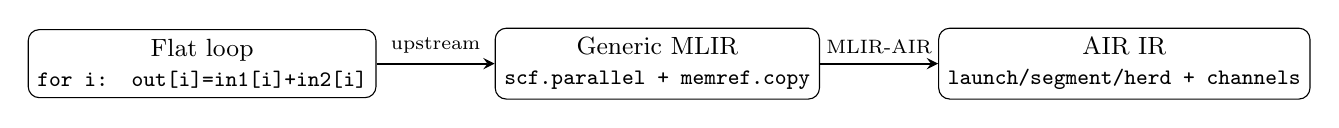
\begin{tikzpicture}[
    stage/.style={rectangle, draw, rounded corners, minimum width=3.5cm,
                  minimum height=0.8cm, font=\small, align=center},
    arr/.style={->, thick, >=stealth},
]
\node[stage] (s0) {Flat loop\\{\footnotesize\texttt{for i: out[i]=in1[i]+in2[i]}}};
\node[stage, right=1.5cm of s0] (s1) {Generic MLIR\\{\footnotesize\texttt{scf.parallel + memref.copy}}};
\node[stage, right=1.5cm of s1] (s2) {AIR IR\\{\footnotesize\texttt{launch/segment/herd + channels}}};

\draw[arr] (s0) -- (s1) node[midway, above, font=\scriptsize] {upstream};
\draw[arr] (s1) -- (s2) node[midway, above, font=\scriptsize] {MLIR-AIR};
\end{tikzpicture}
\end{center}

The programmer writes Stage~0. Upstream frameworks produce Stage~1. MLIR-AIR
produces Stage~2. The programmer never touches spatial constructs---the compiler
adds all placement, data movement, hierarchy, and dependency information
automatically.


% =============================================================================
\section{Scheduling Constructs}
% =============================================================================

\subsection{The Problem: Where Does Computation Run?}

On a CPU, you write code and the OS schedules it onto cores---you never think about
placement. On a GPU, you write a kernel and the hardware scheduler maps thread blocks
to SMs automatically. On a spatial NPU, neither works:

\begin{itemize}[leftmargin=2em]
  \item There is no OS scheduler---tiles are bare-metal, each with its own instruction
    memory.
  \item There is no hardware thread-block scheduler---the compiler must decide
    \emph{which tiles} run \emph{which code} at \emph{which time}.
  \item Resources (tiles, L2 memory, DMA engines) must be explicitly reserved and
    released---no automatic sharing.
\end{itemize}

AIR solves this with a three-level hierarchy that mirrors the physical hardware:
\textbf{launch} (host $\leftrightarrow$ accelerator) $\supset$ \textbf{segment}
(resource pool with L2) $\supset$ \textbf{herd} (compute grid with L1). Think of
it as: \textbf{job $\rightarrow$ department $\rightarrow$ team}.

\subsection{\texttt{air.launch} --- Host-to-Accelerator Boundary}

\textbf{Plain English}: ``send this work to the NPU.'' Like CUDA's
\texttt{kernel<<<>>>} launch, but for spatial hardware. Everything inside runs on
the accelerator; everything outside stays on the host CPU.

\textbf{Key properties:}
\begin{itemize}[leftmargin=2em]
  \item \textbf{Optional iteration space}: multiple independent instances. ``Completely
    parallel schedule is legal'' and instances ``must not rely on observing the effects
    of any other instance'' (p.9).
  \item \textbf{Multiple compiled variants}: compiler emits different versions for
    different resource availability. ``Our lowering for AMD NPU architecture uses
    this freedom to offer different opportunistic granularities (e.g., one column or
    whole array)'' (p.10).
  \item \textbf{Resource lifetime management}: once nested ops finish, launch releases
    hardware resources back to runtime.
\end{itemize}

\subsection{\texttt{air.segment} --- Resource Reservation}

\textbf{Plain English}: ``reserve this chunk of the NPU for my work.'' A segment
claims a pool of tiles + their shared L2 memory + the DMA engines connecting them.
While a segment holds these resources, no other segment can use them. When the
segment finishes, resources are released.

Think of it as booking a conference room: you get the room (L2 memory), the chairs
inside (tiles), and the whiteboard (DMA engines). Others can't walk in until you
leave.

Reserves a \textbf{pool of compute resources} with physical affinity. Groups cores
that share L2 memory and local interconnects.

\textbf{Why separate from herd?} ``An architecture might want to define two pools of
resources that have physical affinity (e.g., resources in one chiplet) so that they
can ensure that the scheduler dispatches \texttt{air.herd} operations within that
segment exclusively using the segment resources'' (p.10).

\textbf{Optional grid space} for replication: \texttt{air.segment [2]} = two identical
resource pools dispatched concurrently (e.g., left and right half of NPU).

\subsection{\texttt{air.herd} --- Parallel Workers on Physical Cores}

\textbf{Plain English}: ``run this code on a grid of tiles simultaneously.'' If
\texttt{air.launch} is ``send work to NPU'' and \texttt{air.segment} is ``reserve
resources,'' then \texttt{air.herd} is ``now actually do the computation on these
specific tiles.'' Every worker in the herd runs the same code body but is
specialized by its tile coordinates---just like CUDA threads use
\texttt{threadIdx} to pick their slice of work.

Group of workers executing concurrently on a grid of compute tiles. Closest analog:
CUDA thread blocks, but with physical placement guarantees that CUDA doesn't give.

\textbf{Key properties:}
\begin{itemize}[leftmargin=2em]
  \item \textbf{Index space}: worker coordinates \texttt{(\%x, \%y)} like CUDA
    \texttt{threadIdx}. Same code, specialized by index.
  \item \textbf{Atomic scheduling}: ``only scheduled when resources for \emph{all}
    the workers are available'' (p.10). No partial herds---avoids deadlocks.
  \item \textbf{Physically contiguous}: ``workers are allocated as a physically local
    contiguous block'' (p.10). 4$\times$2 herd = 4$\times$2 rectangle of adjacent tiles.
    Enables cascade (neighbor-to-neighbor) communication.
  \item \textbf{Multiple herds default sequential}: use \texttt{air.token} to make
    concurrent if desired.
\end{itemize}

\subsection{Hierarchy Maps to Memory Hierarchy}

\begin{center}
\begin{tabular}{lll}
\toprule
\textbf{AIR construct} & \textbf{Scope} & \textbf{Memory level} \\
\midrule
\texttt{air.launch} & Host $\leftrightarrow$ accelerator & L3 / DRAM \\
\texttt{air.segment} & Resource pool & L2 (memory tiles) \\
\texttt{air.herd} & Compute grid & L1 (core scratchpad) \\
\bottomrule
\end{tabular}
\end{center}


% =============================================================================
\section{Data Locality Constructs}
% =============================================================================

\subsection{The Problem: No Caches, No Automatic Data Movement}

On a CPU, when your code reads \texttt{array[i]}, the cache hierarchy transparently
fetches the data from DRAM into L3, then L2, then L1---you never think about it.
On a GPU, shared memory (\texttt{\_\_shared\_\_}) requires manual management, but
global memory accesses are still cached.

On a spatial NPU, \textbf{there are no caches at all}. Each tile has a small
scratchpad (L1, typically 32--64\,KB). Shared memory tiles provide L2. DRAM sits
behind shim tiles at the edge of the array. If your compute tile needs data, someone
must explicitly:
\begin{enumerate}[leftmargin=2em]
  \item Program a DMA engine to copy data from DRAM into L2
  \item Program another DMA to copy from L2 into the tile's L1 scratchpad
  \item After compute, reverse the process for results
\end{enumerate}

The compiler must express all of this explicitly in the IR. AIR provides three
levels of abstraction for this: MemRef annotations (where data lives),
\texttt{air.memcpy} (transitional coupled movement), and \texttt{air.channel}
(the real decoupled primitive).

\subsection{Memory Hierarchy via MemRef Annotations}

\textbf{Plain English}: tag each buffer with \emph{which memory} it lives in.
Standard MLIR \texttt{memref} defaults to global memory. AIR adds memory space
annotations that actually mean something:

\begin{lstlisting}
%global = memref<1024xf32>                    // default: DRAM (L3)
%l2_buf = memref<256xf32, memory_space=L2>    // shared memory tile
%l1_buf = memref<64xf32, memory_space=L1>     // core-local scratchpad
\end{lstlisting}

Three levels mapped to NPU hardware:
\begin{itemize}[leftmargin=2em]
  \item \textbf{L3 / DRAM} --- off-chip, behind shim tiles, huge, slow
  \item \textbf{L2 / cluster scratchpad} --- memory tiles, shared by column of cores
  \item \textbf{L1 / private} --- on compute tile, per-core, small, fastest
\end{itemize}

\subsection{\texttt{air.memcpy} --- Transitional Abstraction}

\textbf{Plain English}: ``copy this data between memory levels, and here's which
levels.'' It's an enhanced \texttt{memref.copy} that carries metadata about
hierarchy levels and data layout. Think of it as an intermediate step---the compiler
uses it while lowering from generic MLIR, before splitting it into decoupled
put/get. You rarely see it in final AIR output.

Key capability: \textbf{in-flight data reshaping}. ``Decoupling the logical layout of
a MemRef from its physical representation in memory'' (p.11). DMA hardware supports
stride-based reshaping---e.g., copy from L3 to L2 while rearranging row-major to
tiled layout.

\texttt{air.memcpy} is intermediate; lowered to \texttt{air.channel} operations:
\begin{lstlisting}
air.memcpy (%src, %dst)           // high level
    // lowered to:
air.channel.put @chan (%src)       // decouple into put + get
air.channel.get @chan (%dst)
\end{lstlisting}

\subsection{\texttt{air.channel} --- Core Data Movement Primitive}

\textbf{Plain English}: the real way data moves on the NPU. Instead of one
\texttt{memcpy} that names both source and destination (coupled), you split it:
one actor \texttt{put}s data onto a named channel, another actor \texttt{get}s
from that channel. They don't name each other---just the channel. This is like a
conveyor belt: the warehouse puts boxes on, the factory floor takes boxes off.
Neither knows or cares about the other's internals.

Stream-based transfer between distinct memory regions. Decoupled into a \texttt{put}
(producer) and \texttt{get} (consumer) linked through a named symbolic channel.

From p.11:
\begin{itemize}[leftmargin=2em]
  \item \textbf{\texttt{put}}: transfers data from a source address onto a serialized
    stream
  \item \textbf{\texttt{get}}: retrieves data from the stream into a destination
    address at a particular memory level
\end{itemize}

\textbf{Why decouple into put/get instead of one memcpy?}

\begin{enumerate}[leftmargin=2em]
  \item \textbf{Producer and consumer live at different hierarchy levels.}
    The \texttt{put} sits in the segment body (L2 scope), the \texttt{get} inside the
    herd body (L1 scope). Each op is local to its memory scope:
\begin{lstlisting}
air.segment {
    %l2_buf = memref.alloc() : memref<256xf32, L2>
    air.channel.put @chan (%l2_buf)     // L2 scope

    air.herd [%x, %y] in [4, 1] {
        %l1_buf = memref.alloc() : memref<64xf32, L1>
        air.channel.get @chan (%l1_buf) // L1 scope
        // compute on l1_buf
    }
}
\end{lstlisting}

  \item \textbf{Cross-level references.} A \texttt{put} at launch level (L3) can
    feed a \texttt{get} inside a herd (L1). The channel abstracts however many hops
    the data takes.

  \item \textbf{Independent optimization.} Compiler can schedule put early
    (prefetch), delay get, optimize each side's DMA path independently.
\end{enumerate}

\textbf{Broadcasting:} One \texttt{put} feeds multiple \texttt{get}s. Specified
through affine integer sets mapping source to destination indices. Lowers to NoC
multicast on AMD NPU.

\textbf{Channel bundles:} Group related channels---e.g.,
\texttt{@chan\_A[0]}, \texttt{@chan\_A[1]} for different tiles of matrix A.

\textbf{MemRef integration:} \texttt{air.channel} ops use same offset/size/stride
semantics as standard MLIR, so existing analysis passes still work.

\subsection{How Scheduling and Data Locality Interact}

Where data ops appear in the hierarchy tells the compiler which memory level they
operate on:

\begin{lstlisting}
air.launch {                                     // L3 boundary
    air.channel.put @chan_in (%dram_buf)          // L3 -> stream

    air.segment {                                // L2 boundary
        %l2 = memref.alloc() : memref<..., L2>
        air.channel.get @chan_in (%l2)            // stream -> L2
        air.channel.put @chan_local (%l2)         // L2 -> stream

        air.herd [%x, %y] in [4,1] {             // L1 boundary
            %l1 = memref.alloc() : memref<..., L1>
            air.channel.get @chan_local (%l1)     // stream -> L1
            // compute on %l1
        }
    }
}
\end{lstlisting}

Data cascades L3 $\rightarrow$ L2 $\rightarrow$ L1. Each transfer is a separate
put/get pair at the right scope. Compiler sees the full picture: can optimize each
level independently, pipeline transfers across levels, detect broadcast opportunities.

Additionally, \texttt{air.herd} guarantees physical contiguity---neighboring workers
can write to each other's local memory via cascade connections without going through
L2 (p.12). And \texttt{air.segment} ensures ``accesses to shared memories remain
localized within their data producers and consumers, reducing unnecessary data
movement'' (p.12).


% =============================================================================
\section{Synchronization Constructs (Complete)}
% =============================================================================

Two constructs handle synchronization in AIR: \texttt{air.token} (explicit dependency
edges) and \texttt{air.channel} (implicit back-pressure sync). They work at different
levels and complement each other.

\subsection{\texttt{air.token} --- Explicit Dependency Control}

When any operation is marked \texttt{async}, it returns an \texttt{air.token} SSA
value signaling its completion. This token can then be consumed by other operations
to express ``don't start until this finishes'' (Section~5.3.1, p.12).

\textbf{Granularity is tunable.} Paper p.12: ``fine-grained control over execution
dependencies in asynchronous workloads, with the granularity tunable from
coarse-grained synchronization over regions of code to fine-grained per-operation
scheduling.'' You can put one token on an entire \texttt{air.launch} (coarse) or one
per individual DMA op (fine).

\subsubsection{Mechanism 1: \texttt{air.wait\_all} --- Blocking Barrier}

Paper p.12: ``explicit \texttt{air.wait\_all} operations, can be inserted into
synchronous control flow. This allows us to prevent further operation dispatch until
tokens specified in the \texttt{air.wait\_all} operation have signaled completion.''

\begin{lstlisting}
%tok0 = air.channel.get async @chanA, %bufA
%tok1 = air.channel.get async @chanB, %bufB
air.wait_all [%tok0, %tok1]          // BLOCKS until both DMAs done
linalg.matmul %bufA, %bufB, %bufC    // only runs after wait passes
\end{lstlisting}

This is a hard barrier---nothing after it executes until all listed tokens fire.
Simple but conservative.

\subsubsection{Mechanism 2: Synchronization Lists --- Scheduling Graph}

Paper p.12: ``synchronization lists, that explicitly specify the relative scheduling
of operations in time and space, describe a scheduling graph. Backend lowerings can
use this graph to push dependency resolution to distributed dispatchers in hardware
devices.'' Instead of one blocking wall, you build a graph of ``who waits for whom''
that the hardware scheduler interprets directly.

\subsection{Three Types of Synchronization Edges}

The compute model defines three types of relationships between operations (p.12):

\subsubsection{Dependency Lists --- Directed, ``Happens-Before''}

Paper p.12: ``Dependency lists encode directed edges between an operation and the
predecessor operations in which its inputs are defined. It requires that all inputs
to an operation that are modified by a source operation in the dependency list are
visible before the sink operation is scheduled.''

\begin{lstlisting}
%tok0 = air.channel.get async ...        // DMA writes bufA
%tok1 = linalg.matmul async [%tok0] ...  // dep list: [%tok0]
// tok1 can't start until tok0 finishes (RAW dependency)
\end{lstlisting}

This encodes RAW/WAR/WAW hazards as directed edges in the ACDG.

\subsubsection{Concurrency Lists --- Undirected, ``Must Co-Schedule''}

Paper p.12: ``Each \texttt{air.token} in a concurrency list defines an undirected
edge between two operations that indicates they must be scheduled at the same time.
This implies that each operation must use exclusive resources.''

This is for \emph{guaranteeing} overlap, not just allowing it. Example: double
buffering where DMA fills buffer B while compute processes buffer A. You want to
\emph{require} they run simultaneously on separate resources (separate DMA engine
and compute unit).

\subsubsection{Affinity Lists --- Undirected, ``Same Resources, Different Time''}

Paper p.12: ``These are lists of tokens that define undirected edges between
operations that must execute using the same resources. In practice, this means
these operations' time-slots must be disjoint, but the edge does not describe
which operation must be scheduled first.''

Opposite of concurrency: these ops share a resource (e.g., same DMA engine), so
they can't overlap, but either could go first. The affinity edge says ``same
resource, you figure out the order.''

\subsection{Tokens in Loops}

\subsubsection{\texttt{scf.for} --- Single Token (Fig~4a)}

One token carried across iterations. Fully sequential---each iteration waits for
the previous one's entire body:

\begin{lstlisting}
%tf = scf.for %i = 0 to %N iter_args(%ta) {
    %t1 = air.op async [%ta]
    %t2 = air.op async [%t1]
    scf.yield %t2   // pass to next iteration
}
\end{lstlisting}

\subsubsection{\texttt{scf.for} --- Multiple Tokens (Fig~4b)}

Paper p.17: ``An arbitrary number of \texttt{air.token} values can be carried
across iterations, each representing an independently progressing thread of
execution.''

\begin{lstlisting}
%tf = scf.for %i iter_args(%ta, %tb, %tc, %td) {
    %t1 = air.op async [%ta, %tc]
    %t2 = air.op async [%t1, %td]
    %t3 = air.op async [%ta, %t1]
    %t4 = air.op async [%t1, %t2]
    scf.yield %t1, %t2, %t3, %t4  // four independent streams
}
\end{lstlisting}

Four independent dependency chains flowing across iterations. Some chains from
iteration $i{+}1$ can start while others from iteration $i$ still run. Paper p.17:
``This enables precise modeling of parallel pipelines, race conditions, and shared
resource usage.''

\subsubsection{\texttt{scf.parallel} --- Fork/Join (Fig~4c)}

Paper p.17: ``MLIR-AIR supports asynchronous dependencies within structured
parallel execution constructs such as \texttt{scf.parallel}.''

\begin{lstlisting}
%init = air.wait_all async
%tp = scf.parallel (%i) = (0) to (%N) init (%t1) {
    %td = air.memcpy async [%t1] (%y[%i], %a[%i])
    %tc = air.op async [%td]
    scf.reduce(%tc) {
        ^bb0(%lhs, %rhs):
        %tj = air.wait_all async [%lhs, %rhs]
        scf.reduce.return %tj
    }
}
\end{lstlisting}

Key points:
\begin{itemize}[leftmargin=2em]
  \item \textbf{Synchronized start}: \texttt{air.token} in init argument starts all
    parallel threads together
  \item \textbf{Synchronized end}: \texttt{air.wait\_all} reduction tree collects all
    tokens---all iterations must finish before the region completes
  \item \textbf{Within each iteration}: async dependencies work normally
\end{itemize}

\subsection{\texttt{air.channel} as Synchronization}

Channels are not just data movement---they also synchronize (Section~5.3.2, p.13).

Paper p.13: ``an \texttt{air.channel.get} operation is synchronized to an
\texttt{air.channel.put} with the same \texttt{air.channel} by back pressure.''

\textbf{Back pressure} means: the channel is a bounded buffer. If the producer pushes
data and the consumer hasn't consumed previous data, the producer \textbf{stalls}.
No explicit token needed---the channel itself enforces ordering:

\begin{lstlisting}
// In segment body:
air.channel.put @chan (%l2_data)    // pushes data

// In herd body:
air.channel.get @chan (%l1_buf)     // implicitly waits for put
// No token connects these -- @chan IS the sync mechanism
\end{lstlisting}

Paper p.13: ``This synchronization abstraction---combined with asynchronous
dependencies on \texttt{air.channel} actors to enforce synchronization local to each
memory space---is both simple and effective: enforcement of dependencies between
distributed data movers does not require complex control-flow dependencies across
code regions.''

Without channel back-pressure, you'd need explicit tokens crossing from segment
scope into herd scope. Channel back-pressure handles it implicitly.

\subsection{Grouped Completion via \texttt{air.launch}}

Paper p.13: ``an \texttt{air.launch}'s \texttt{air.token} is released only when
\emph{all} operations within the \texttt{air.launch} have completed.''

\texttt{air.launch} produces a single token that fires when everything inside
(segments, herds, DMAs) finishes. The host synchronizes on ``entire accelerator job
done'' without tracking individual ops.

\subsection{Hardware Pipelining: Ping-Pong Buffering}

Section~7.4.1 (p.20) describes the concrete payoff. The loop is unrolled by 2,
yielding ``ping'' and ``pong'' threads with four loop-carried tokens:
\begin{itemize}[leftmargin=2em]
  \item 2 tokens for producer-consumer dataflow (ping stage and pong stage)
  \item 2 tokens for intra-stage resource contention (producer-side and consumer-side)
\end{itemize}

The flattened ACDG (Fig~7, p.20) shows the interleaved pipeline:

\begin{center}
\begin{tabular}{ll}
\toprule
\textbf{Time} $\rightarrow$ & \\
\midrule
Ping: & \texttt{[produce]} $\rightarrow$ \texttt{[consume]} $\rightarrow$
  \texttt{[produce]} $\rightarrow$ \texttt{[consume]} \\
Pong: & \qquad\texttt{[produce]} $\rightarrow$ \texttt{[consume]} $\rightarrow$
  \texttt{[produce]} $\rightarrow$ \\
\bottomrule
\end{tabular}
\end{center}

While ping consumer processes data, pong producer fills next buffer. Paper p.20
validates: ``data reads and writes execute concurrently across two buffers,
validating the correctness and effectiveness of the pipelined ACDG transformation.''

\subsection{Synchronization Summary}

\begin{center}
\small
\begin{tabular}{llll}
\toprule
\textbf{Mechanism} & \textbf{Type} & \textbf{Scope} & \textbf{How} \\
\midrule
Token + dep list & Explicit, directed & Any ops & A before B \\
Token + concurrency & Explicit, undirected & Co-scheduled & Must overlap \\
Token + affinity & Explicit, undirected & Resource-sharing & Same resource, no overlap \\
\texttt{air.wait\_all} & Explicit barrier & Sync flow & Block until all fire \\
Channel back-pressure & Implicit & Cross-hierarchy & Get waits for put \\
Launch completion & Implicit group & Host boundary & Fires when all inside done \\
\bottomrule
\end{tabular}
\end{center}

Tokens are the \textbf{fine-grained} mechanism (per-operation). Channels are the
\textbf{cross-hierarchy} mechanism (across segment/herd boundaries). Together they
express any pattern from fully sequential to deeply pipelined, and backend lowerings
push it all to hardware dispatchers.


% =============================================================================
\section{Summary: The AIR Mental Model}
% =============================================================================

\begin{center}
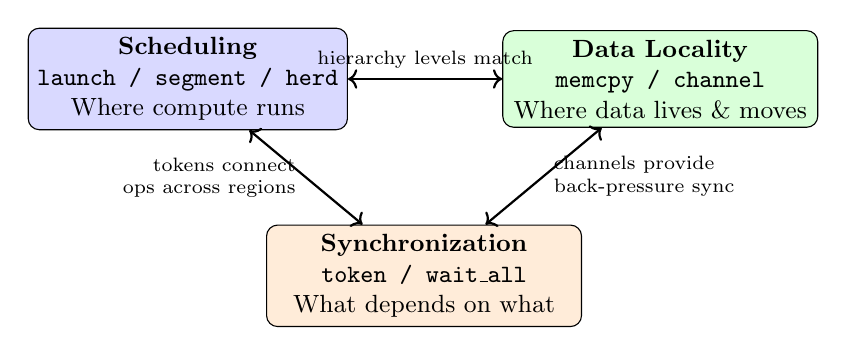
\begin{tikzpicture}[
  concept/.style={draw, rounded corners, fill=#1, minimum width=4cm,
    minimum height=1cm, align=center, font=\small},
  arrow/.style={-{Stealth}, thick},
]
\node[concept=blue!15] (sched) at (0,0) {\textbf{Scheduling}\\
  \texttt{launch / segment / herd}\\Where compute runs};
\node[concept=green!15] (data) at (6,0) {\textbf{Data Locality}\\
  \texttt{memcpy / channel}\\Where data lives \& moves};
\node[concept=orange!15] (sync) at (3,-2.5) {\textbf{Synchronization}\\
  \texttt{token / wait\_all}\\What depends on what};

\draw[arrow, <->] (sched) -- (data)
  node[midway, above, font=\scriptsize] {hierarchy levels match};
\draw[arrow, <->] (sched) -- (sync)
  node[midway, left, font=\scriptsize, align=right] {tokens connect\\ops across regions};
\draw[arrow, <->] (data) -- (sync)
  node[midway, right, font=\scriptsize, align=left] {channels provide\\back-pressure sync};
\end{tikzpicture}
\end{center}

These three categories of constructs together let AIR represent:
\begin{itemize}[leftmargin=2em]
  \item \textbf{Concurrency control} --- which cores run what, when
  \item \textbf{Memory placement} --- which data lives where in the hierarchy
  \item \textbf{Data movement} --- explicit DMA ops, visible and schedulable
  \item \textbf{Synchronization} --- explicit dependency edges, not implicit ordering
\end{itemize}

All as first-class, compiler-visible operations in the MLIR framework.

\end{document}
